\clearpage
\section{Appendix}

\subsection{Horizontal prototype}
\label{horizontal-prototype}

\begin{figure}[h!]
    \centering
    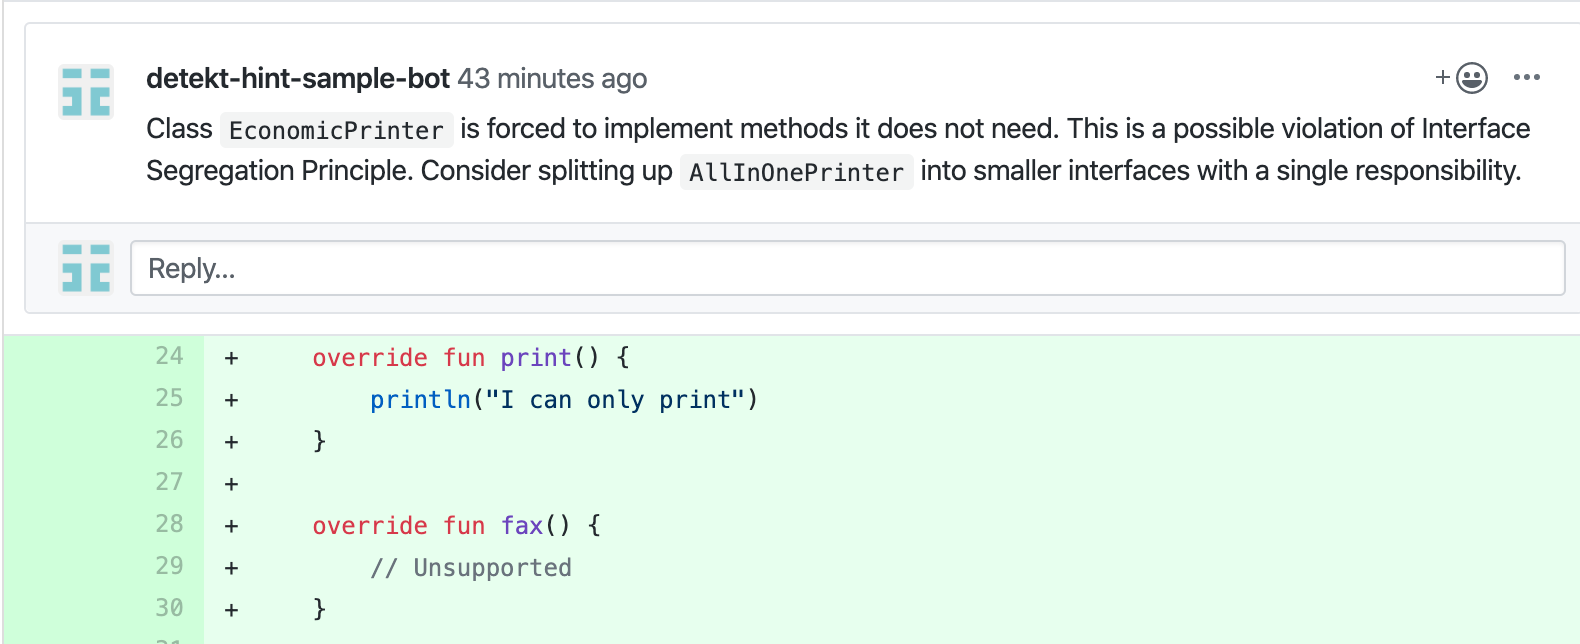
\includegraphics[width=\textwidth]{../comment_isp.png}
    \caption{Prototype of the \gls{isp} rule }
    \label{fig:isp}
\end{figure}


\begin{figure}[h!]
    \centering
    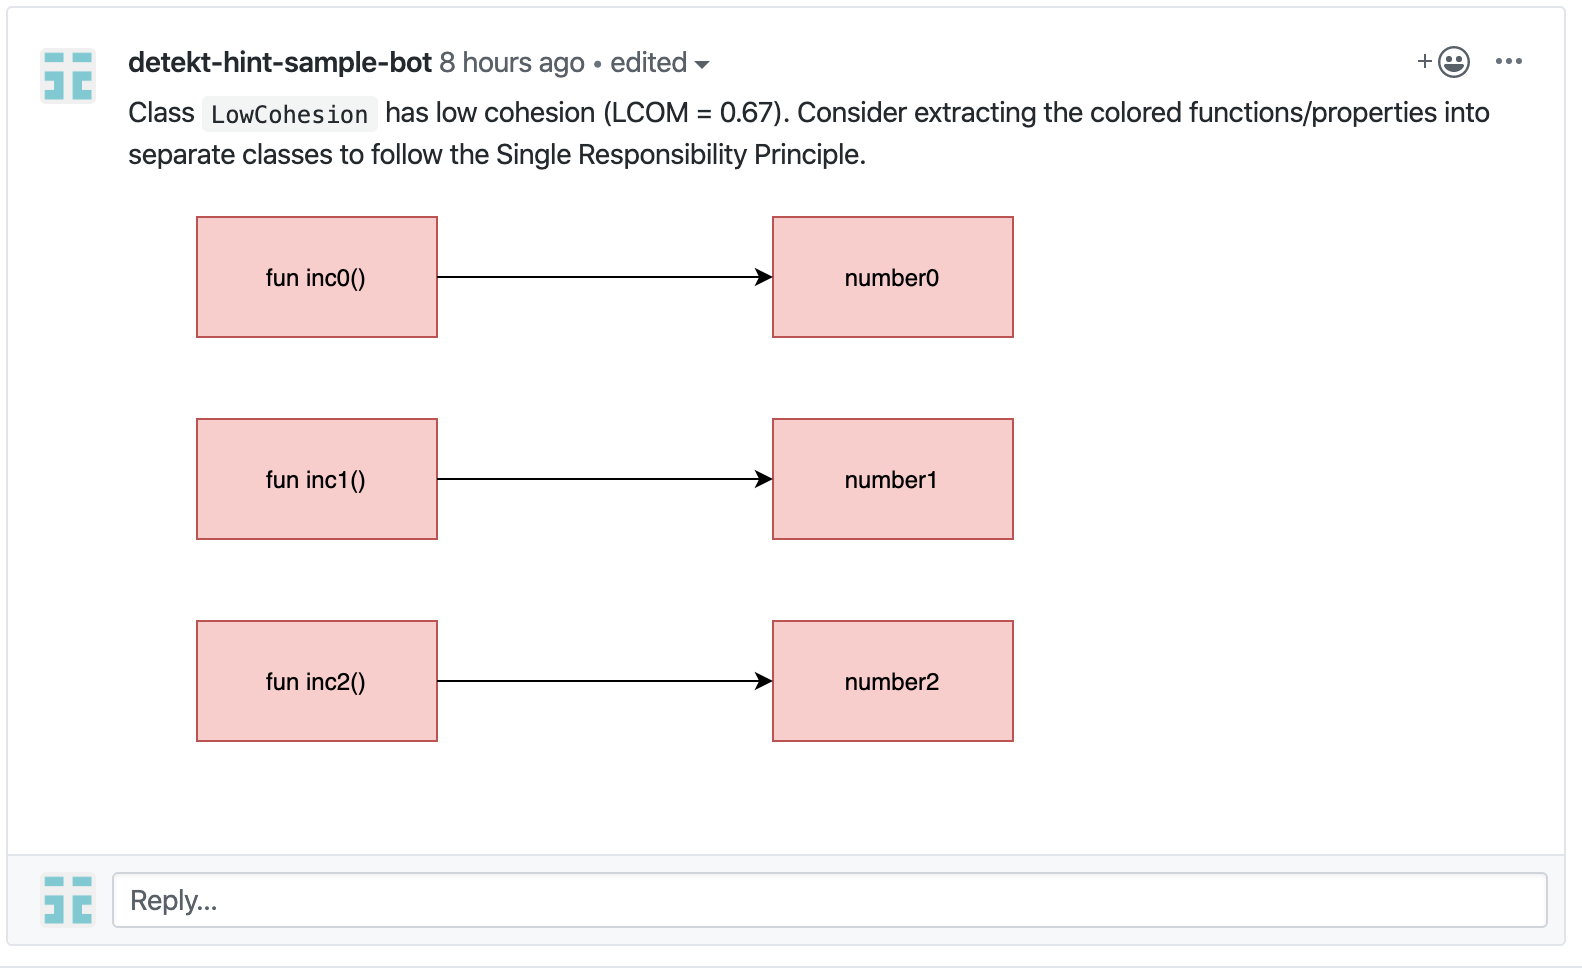
\includegraphics[width=\textwidth]{../comment_lackOfCohesion.png}
    \caption{Prototype of the \gls{lcom} rule}
    \label{fig:lcom}
\end{figure}


\begin{figure}[h!]
    \centering
    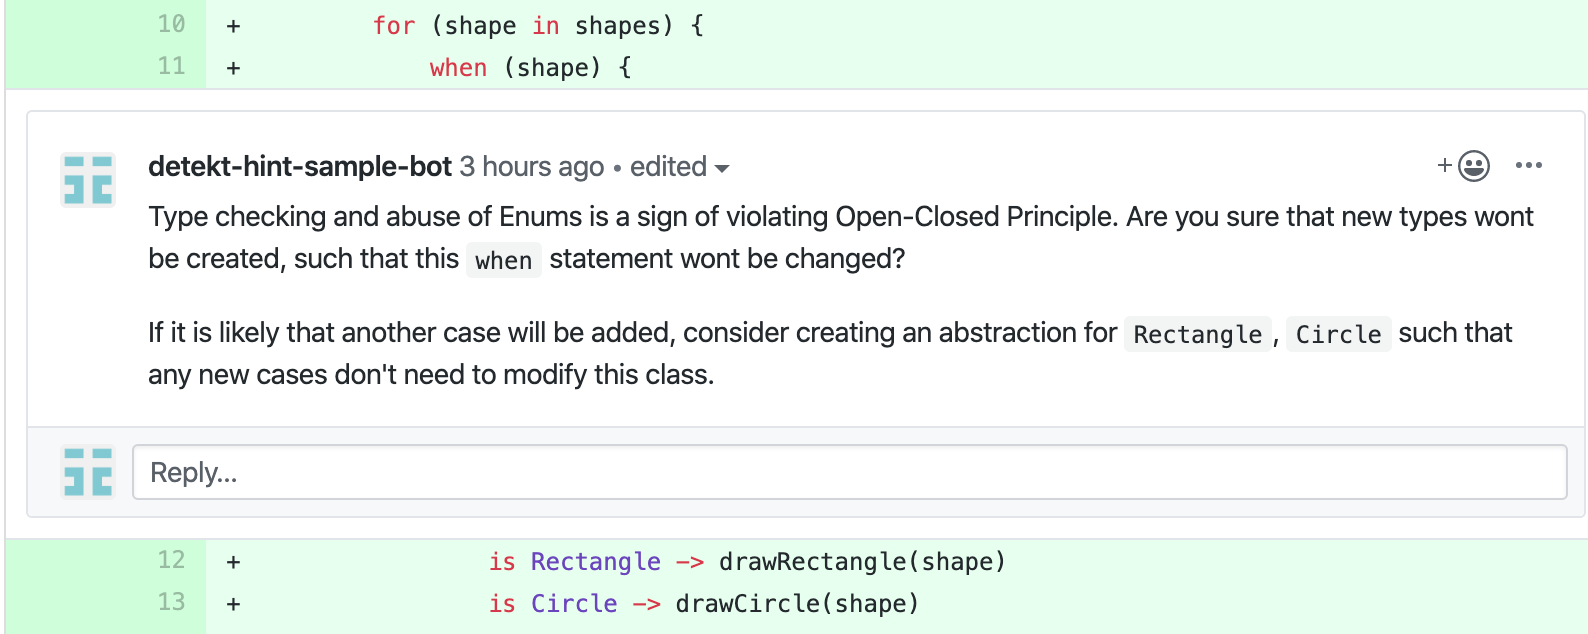
\includegraphics[width=\textwidth]{../comment_ocp.png}
    \caption{Prototype of the \gls{ocp} rule}
    \label{fig:ocp}
\end{figure}


\begin{figure}[h!]
    \centering
    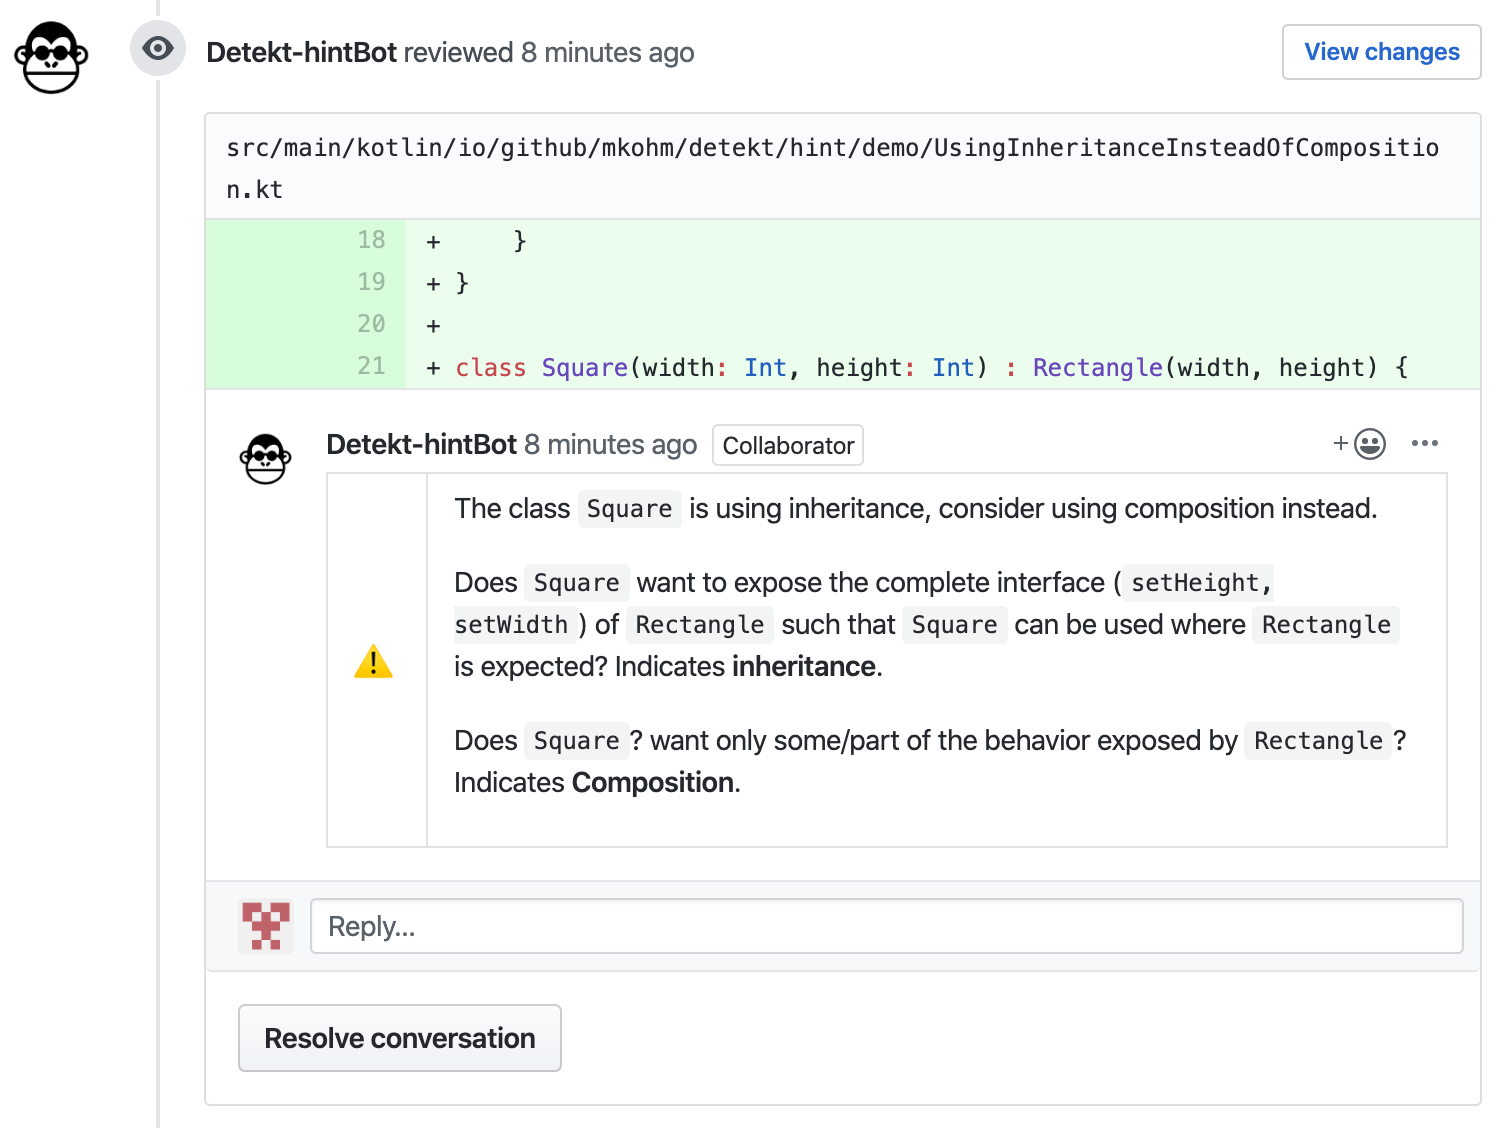
\includegraphics[width=\textwidth]{../demo.png}
    \caption{Prototype of the composition over inheritance / \gls{lsp} rule}
    \label{fig:liskov}
\end{figure}

\clearpage

\subsection{Horizontal prototype schema}
\subsubsection*{Participant} What is the name of the participant.
\subsubsection*{Background:} What is the participants background. Experience with software architecture? Knows and uses design principles? Experience with Kotlin?
\subsubsection*{Presentation of rules - For each rule}
\begin{enumerate}
    \item Present the rule. 
    \item Make sure the participant understands the importance of the rule.
    \item When will the rule give a warning?
    \item When will the rule incorrectly give a warning? Will it report false-positives too often? Suggestions on how to reduce the amount?
    \item How much context is needed? Shorter or longer comments? Should include suggestions on possible solutions? Is the comment understandable? Something missing?
\end{enumerate}

\subsubsection*{Other} 
- When reviewing code, what do you think is tedious, and could it be automated?
- Are there any rules/principles missing?

 
\subsection{Horizontal prototype results}
\textbf{Participant:} Eirik Vale Aase \newline
\textbf{Background:} Studies computer science at \gls{ntnu} with a specialization in computers and systems software. Has experience with developing apps for iOS and web development. Interested in Software Architecture and writing software of high quality. \\
Rule - UseCompositionInsteadOfInheritance:
Present the rule. Make sure the participant understands the importance of the rule. When will the rule give a warning? When will the rule incorrectly give a warning?
Initial thoughts:
Is it useful?

\clearpage
\subsection{Workshop schema}
\label{workshop-schema}


\subsection{Pre-study}
\todo{Add pre study as appendix}
